\section{Architettura del prodotto}
\subsection{Descrizione generale}
Il pattern architetturale scelto dal gruppo per lo sviluppo del progetto è il Model-View-ViewModel. Il seguente pattern è tra i più diffusi nello sviluppo delle web application e permette di scrivere codice facilmente mantenibile e riusabile; questo è possibile grazie al disaccoppiamento lasco che sussiste tra logica di presentazione e di business. Inoltre MVVM è risultato il più adatto per essere utilizzato con React, libreria impiegata per lo sviluppo dell’UI e che renderizza le componenti in base al loro stato interno.
\begin{itemize}
\item \textbf{Model}: questa porzione ricopre la logica di business dell’applicazione, ovvero la gestione dei dati di partenza, dimensioni e strutture create dall’utente ed infine le preferenze di visualizzazione dei grafici. Per una corretta separazione logica, il \textit{Model} è stato suddiviso in tre parti: una dedicata ai dati e alle dimensioni (\textit{Model.js}), una seconda per la gestione delle matrici delle distanze (\textit{DistanceMatricesModel.js}) ed un’ultima dedicata alle preferenze dell’utente (\textit{Preferences.js});

\item \textbf{ViewModel}: qui viene effettuato il \glo{binding} tra \textit{View} e \textit{Model} ed è contenuta la loro logica;

\item \textbf{View}: questa porzione gestisce la presentazione tramite una specifica gerarchia di componenti; ciascun componente contiene la logica strettamente legata alla sua visualizzazione e necessaria al mantenimento del proprio stato interno.
\end{itemize}

Il passaggio dei dati dal \textit{Model} alle varie componenti grafiche avviene attraverso l'utilizzo di un \textit{Context React}, al quale viene passato un'istanza del \textit{ViewModel}. L'utilizzo di un \glo{\textit{Context React}} ci permette di accedere al valore corrente del \textit{ViewModel} in qualsiasi porzione della \textit{View}, senza doverlo passare di componente in componente attraverso le \glo{props}. Nella radice dell'applicazione viene infatti creata un'istanza del \textit{ViewModel}, che viene passata ad un \textit{Context.Provider}, che fa da contenitore per tutta la \textit{View}. All'interno di tale contenitore ogni \glo{component} può utilizzare un \glo{hook} per accedere al \textit{Context React} ed utilizzare il valore più recente del \textit{ViewModel}.\\ È stato scelto di utilizzare un \textit{Context React} per il passaggio dei dati in quanto la nostra applicazione é molto profonda e non risultava conveniente passare i dati per molti componenti rischiando, nel peggiore dei casi, di doverli utilizzare nell'ultimo della gerarchia.\\
Per poter fare in modo che una componente della \textit{View} si renderizzi non solo al cambiamento del suo stato interno ma anche al cambiamento dei dati nel \textit{Model}, abbiamo utilizzato la libreria \glo{\textit{Mobx}}. Questa ci permette di implementare l'\textbf{observer pattern}, non supportato di default da \textit{React}. A tale scopo, Mobx permette di segnare delle classi (o attributi di esse) come "\textit{observable}" e di costruire dei componenti della View come "\textit{observer}". Quest'ultimi vengono automaticamente ri-renderizzati al cambiamento di un qualsiasi attributo \textit{observable}.
\newpage

\subsection{Diagramma dei package}
\begin{figure}[hb]
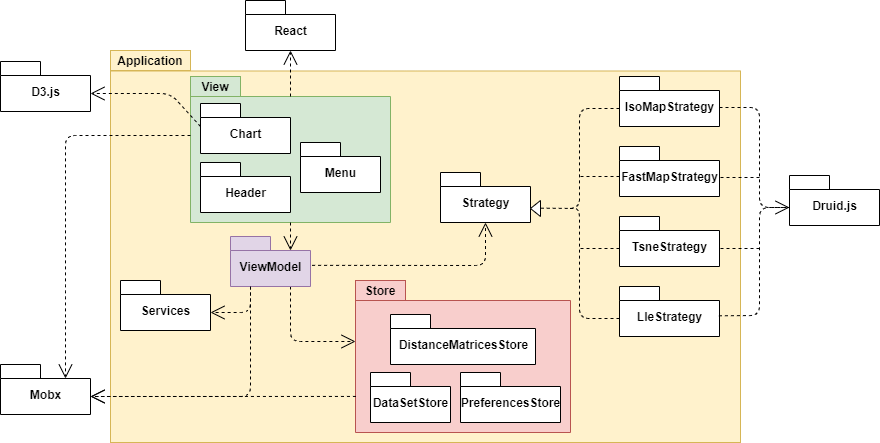
\includegraphics[width=18cm]{Images/Allegato Tecnico-Package}
\centering
\caption{Diagramma dei package del client}
\end{figure}
\begin{figure}[hb]
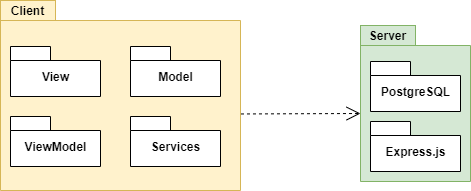
\includegraphics[width=12cm]{Images/Allegato Tecnico-Package 2}
\centering
\caption{Diagramma dei package dell'applicazione}
\end{figure}
\newpage

\subsection{Diagrammi delle classi}
\begin{figure}[hb]
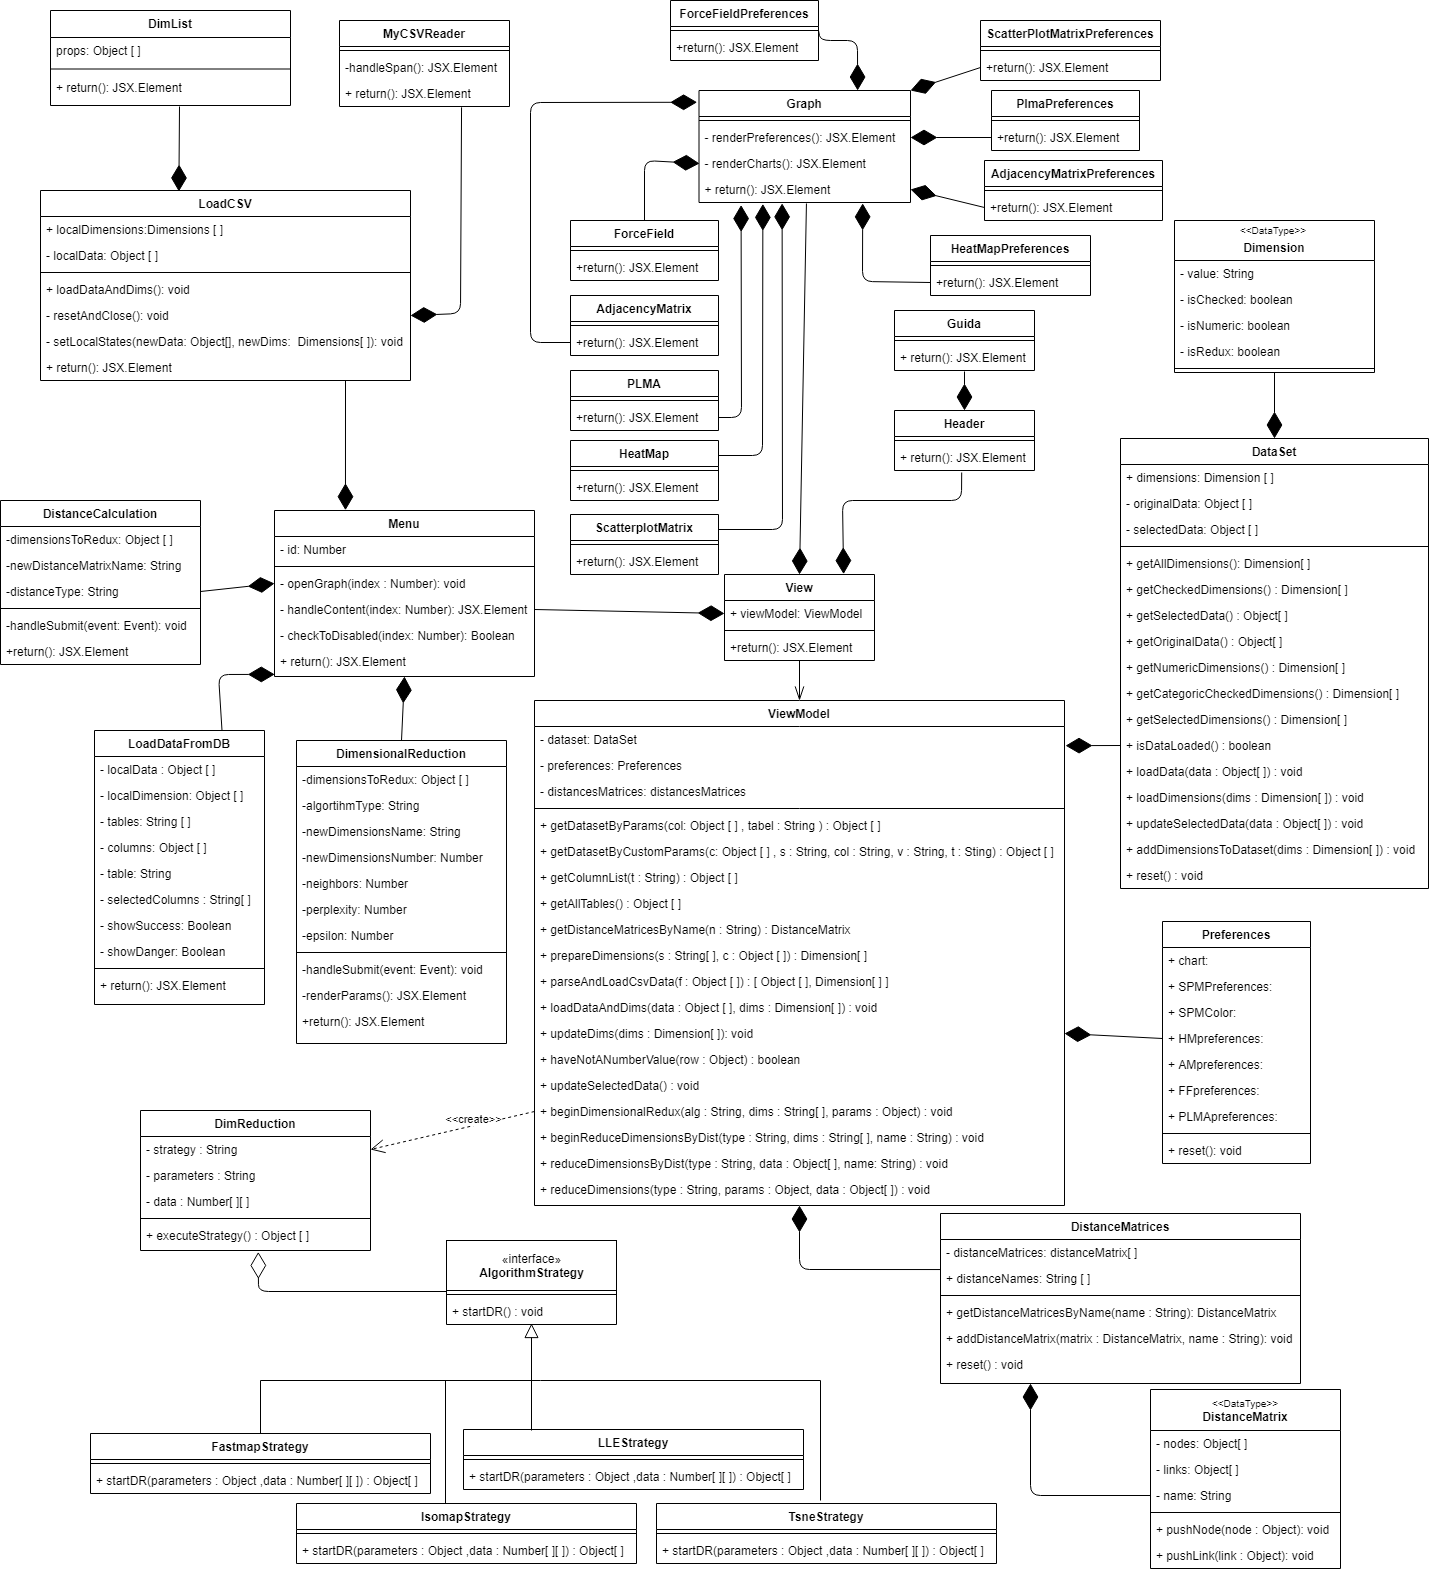
\includegraphics[width=14.8cm]{Images/Allegato Tecnico-Class}
\centering
\caption{Diagramma delle classi generale}
\end{figure}

\begin{landscape}
\vspace*{\fill}
\begin{figure}[hb]
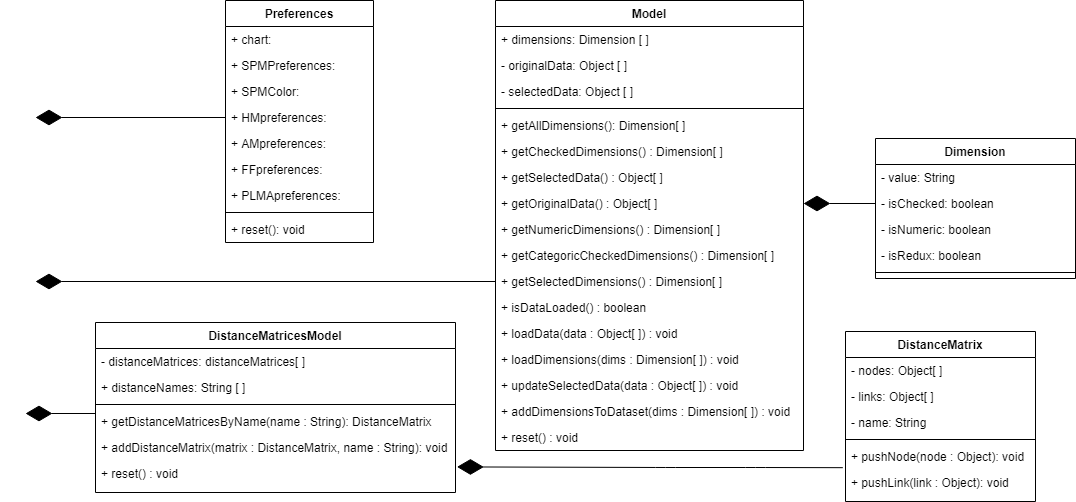
\includegraphics[width=\linewidth]{Images/Allegato Tecnico-Model}
\centering
\caption{Diagramma delle classi, zoom sul modello}
\end{figure}
\vfill
\end{landscape}

\begin{landscape}
\vspace*{\fill}
\begin{figure}[hb]
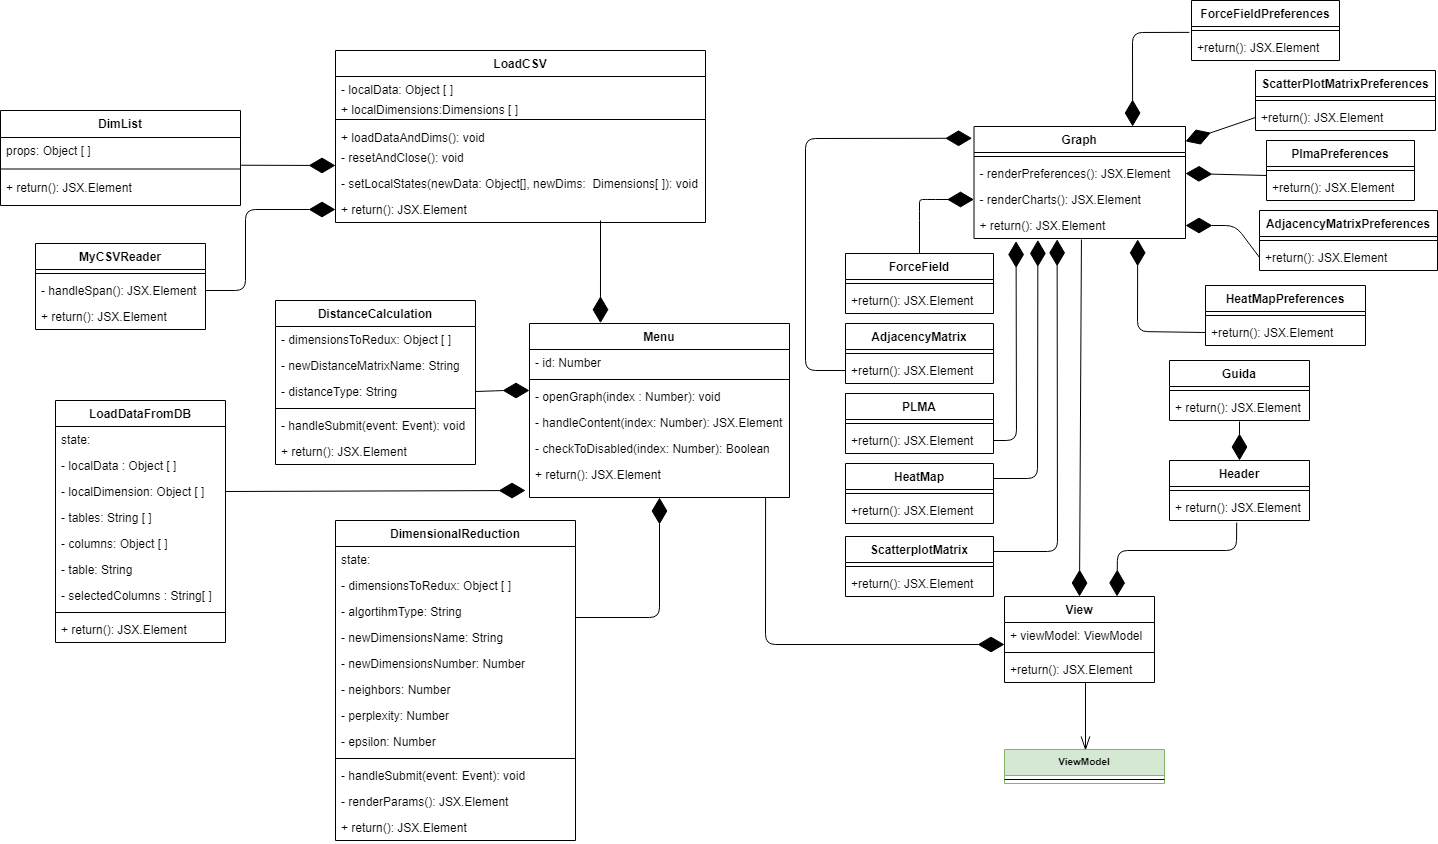
\includegraphics[width=21cm]{Images/Allegato Tecnico-View}
\centering
\caption{Diagramma delle classi, zoom sulla vista}
\end{figure}
\vfill
\end{landscape}

\begin{landscape}
\vspace*{\fill}
\begin{figure}[hb]
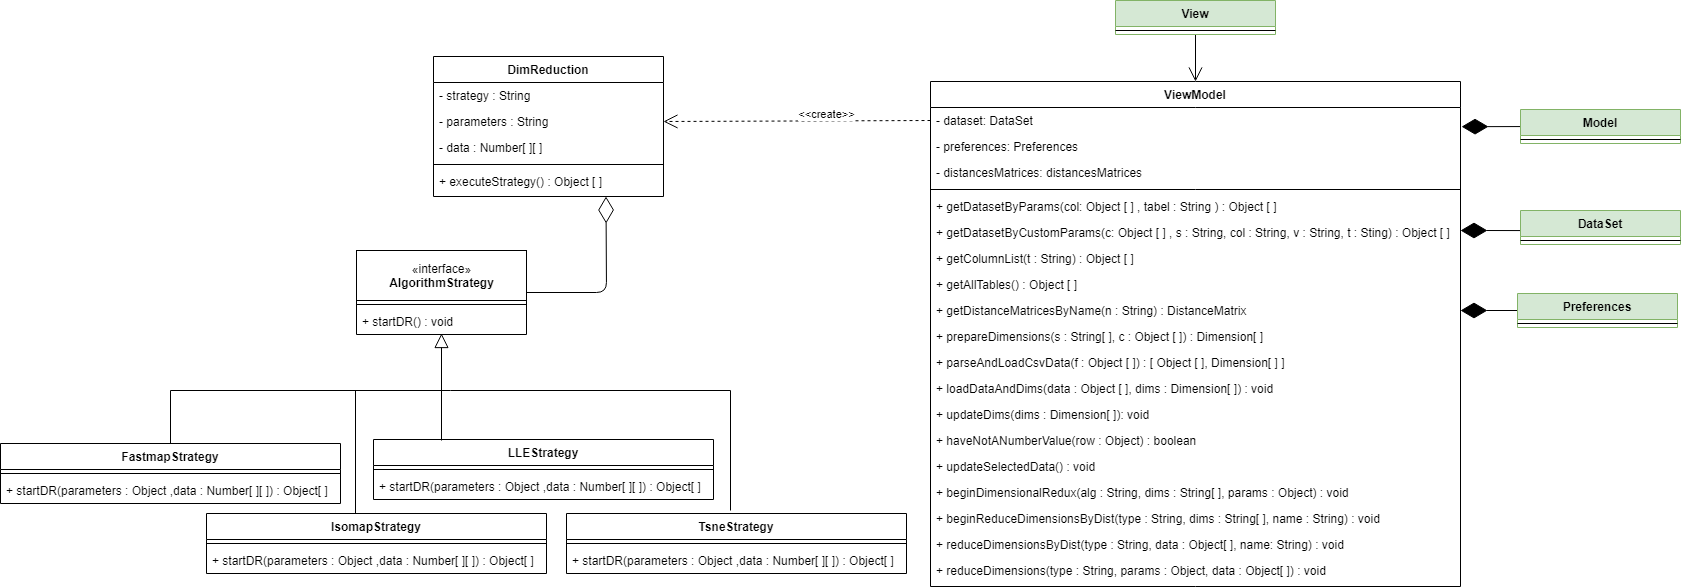
\includegraphics[width=\linewidth ]{Images/Allegato Tecnico-ViewModel}
\centering
\caption{Diagramma delle classi, zoom sul view-model}
\end{figure}
\vfill
\end{landscape}
\newpage
\subsection{Diagrammi di sequenza}
Qui di seguito vengono rappresentati i diagrammi di sequenza per le 3 operazioni più importanti nel progetto:
\begin{figure}[hb]
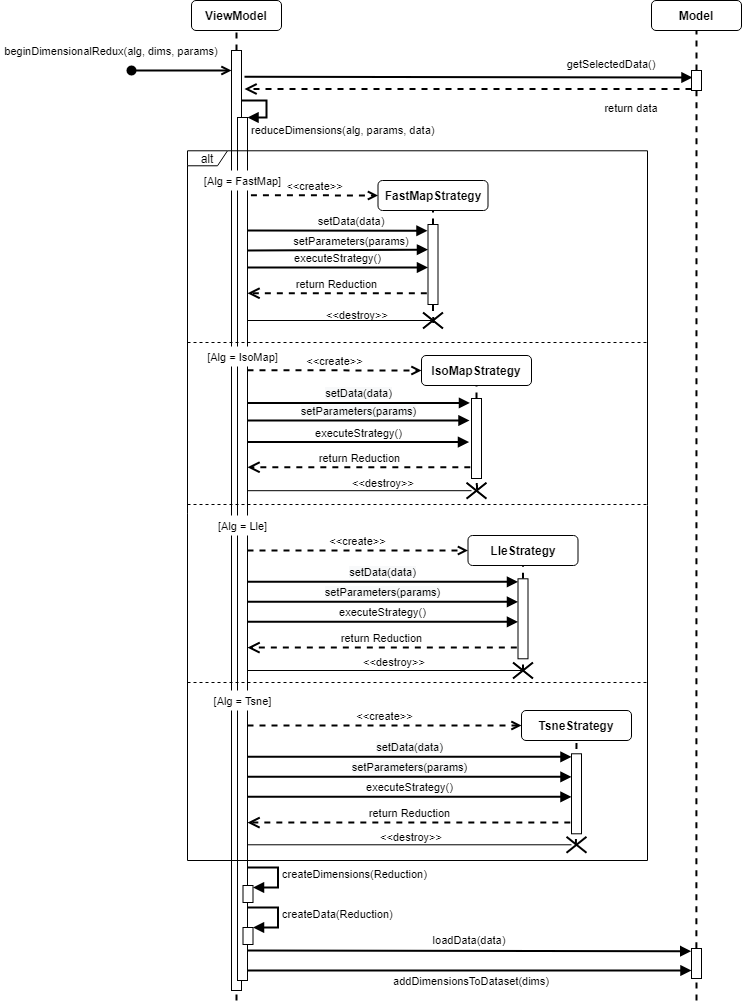
\includegraphics[width=12cm]{Images/Allegato Tecnico-Sequenza-DR}
\centering
\caption{Diagramma di sequenza che modella il processo di riduzione dimensionale}
\end{figure}
\newpage
\begin{figure}[hb]
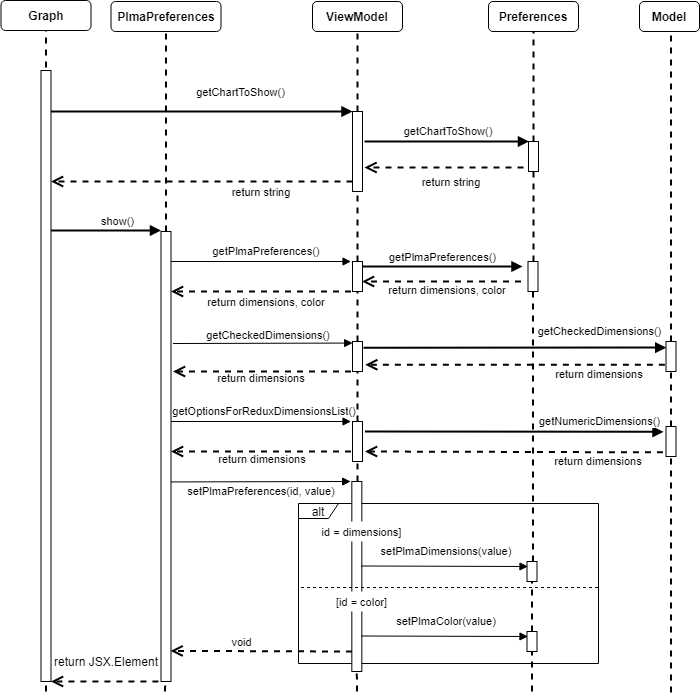
\includegraphics[width=15.5cm]{Images/Allegato Tecnico-Sequenza-PLMApref}
\centering
\caption{Diagramma di sequenza che modella il processo di visualizzazione delle preferenze per il grafico PLMA}
\end{figure}
\newpage
\begin{figure}[hb]
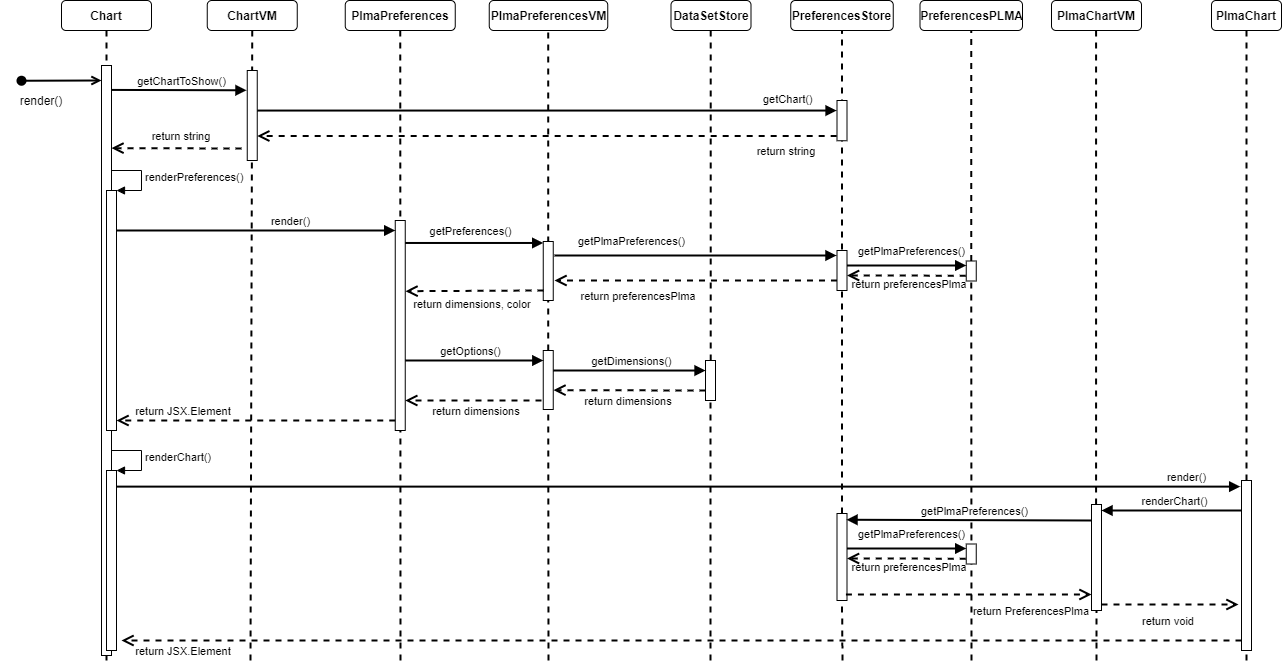
\includegraphics[width=15.5cm]{Images/Allegato Tecnico-Sequenza-PLMA}
\centering
\caption{Diagramma di sequenza che modella il processo per la visualizzazione del grafico PLMA}
\end{figure}
\newpage

\subsection{Design pattern utilizzati}
Per implementare il processo di riduzione dimensionale è stato utilizzato il design pattern \textbf{strategy}. Questo è stato possibile perché l'unica sostanziale differenza era determinata dalla tipologia di algoritmo applicato. Definire una famiglia di algoritmi e isolarli all'interno di un oggetto ci ha permesso di renderli interscambiabili dinamicamente ed evitare duplicazione di codice. 
\begin{itemize}
\item \textbf{DimReduction.js}: rappresenta il \textit{Context}, ovvero la classe concreta che invoca la \textit{ConcreteStrategy} sotto richiesta del client;
\item \textbf{AlgorithmStrategy.js}: interfaccia comune a tutti gli algoritmi ed utilizzata da \textit{DimReduction} per settarli ed invocarli;
\item \textbf{FastmapStrategy.js, IsomapStrategy.js, LLEStrategy.js, TsneStrategy.js}: rappresentano gli algoritmi concreti ed espongono l'interfaccia comune.
\end{itemize}

Nel nostro caso, il pattern si basa sul metodo \textbf{startDR()} che esegue la riduzione dimensionale sui dati scelti e ritorna le nuove dimensioni. La strategy viene passata come stringa e, una volta creata la classe concreta dell'algoritmo scelto, viene costruita l'apposita istanza dalla libreria \textit{Druid.js}.\\Eventuali integrazioni con ulteriori algoritmi di riduzione dimensionale potranno essere effettuate derivando nuove classi concrete dall'interfaccia esposta.